\documentclass{article}
\usepackage{graphicx} 
\usepackage{graphicx, subcaption}% Required for inserting images
\usepackage[ruled,vlined]{algorithm2e}
\usepackage{xcolor} % for colored text
\usepackage{graphicx} % for including graphics
\usepackage{amsmath} % for advanced math features
\usepackage{float}
\usepackage{amssymb}
\usepackage{amsthm}

\title{CS529 Project 1 Report - Group 15}
\vspace{3cm}
\author{
    \begin{tabular}[t]{c@{\hskip 2em}c} % Two columns with some space in between
        Behnoud Alaghband & Zhuoming Liu  \\
        University of New Mexico & University of New Mexico \\
        \texttt{balaghband@unm.edu} & \texttt{dawnmoon@unm.edu}
    \end{tabular}
}


\begin{document}

\maketitle

\section{Data}
\subsection{Data Overview}
The dataset is a 472432 $\times$ 27 matrix, 472432 records and 27 features (columns). Among 27 features, there are 25 explanatory features, 1 target feature ("isFraud"), 1 index feature ("TransactionID"). Except the target feature and index feature, the rest 25 features are classified as numerical or categorical (Table 1).

\begin{table}[H]
    \centering
    \resizebox{1 \textwidth}{!}{
        
        \begin{tabular}{r|r|r|r|r}
            Feature & Numerical & Categorical & \# of Unique values & \% of missing values \\\hline
            ProductCD& & \checkmark & 5 & 0\\
            card1& &\checkmark &12815 & 0\\
            card2& &\checkmark &501 & 1.52\\
            card3& &\checkmark &112 & 0.27\\
            card4& &\checkmark &5 & 0.27\\
            card5& &\checkmark &115 & 0.72\\
            card6& &\checkmark &5 & 0.27\\
            addr1& &\checkmark &304 & 11.09\\
            addr2& &\checkmark &72 & 11.09\\
            c1&\checkmark &&1350 & 0\\
            c2&\checkmark &&1064 & 0\\
            c3&\checkmark &&21 & 0\\
            c4&\checkmark &&1078 & 0\\
            c5&\checkmark &&319 & 0\\
            c6&\checkmark &&1158 & 0\\
            c7&\checkmark &&914 & 0\\
            c8&\checkmark &&1002 & 0\\
            c9&\checkmark &&204 & 0\\
            c10&\checkmark &&987 & 0\\
            c11&\checkmark &&1210 & 0\\
            c12&\checkmark &&927 & 0\\
            c13&\checkmark &&1393 & 0\\
            c14&\checkmark &&1018 & 0\\
            TransactionAmt&\checkmark &&7898 & 0\\
            TransactionDT&\checkmark &&461340 & 0\\
        \end{tabular}
    }
    \caption{ Data overview}
\end{table}
'TransactionDT' has 461340 unique values in our dataset (Table 1), indicating 'TransactionDT' should not be used in the decision tree (DT). Same reason from Micheal's book, 'TransactionDT' can cause a highly over-fitting tree. In fact, 'TransactionDT' is the date of transaction, usually meaningless for determining whether the transaction is fraud or not. Although an organization is faking the transaction in a particular day may happen in some cases, we don't take that situation into consideration. We will ignore 'TransactionDT' when building our Random Forest (RF).

\subsection{Records with "NaN"}
Some records have missing values for a certain feature. Table 2 gives out how many records have missing values in each feature. For example, there are 11.09\% of records have missing values in "addr2" feature.\\
Two strategies were applied in the training phase.
\begin{enumerate}
    \item Remove records
    \\We removed the record if any of its features has a missing value. After the data cleaning, we had 87.17\% records left for use. Obviously, this strategy is very easy for implementation, but it resulted in less data in the training phase, which affected the performance of RF.
    \item Simulate feature value
    \\For the record with a missing feature, we will assign it with the most common feature value from the rest of the dataset. This can keep our records as much as possible. And We won't waste those useful information from the records with missing values. Actually based on Table 1, we can simulate an extremely worst case -- one record has 7 missing feature values (card2 -card6, addr1, addr2). The rest 18 features contain useful information still.
\end{enumerate}
Although intuitively, I thought strategy 2 is the best choice, since it keeps as much records as possible. However, the results from experiments tell a different story (Table 3, \textcolor{red}{more explained in section} ). For the "Gini index", strategy 1 performed better than strategy 2. But for the "Entropy" and "Miss classification", strategy 2 did out-performed strategy 1 with more stable and higher balanced accuracy. Based on these experiments, we choose to use the strategy 1 to deal with missing value in training phase.\\\\
In validation phase, we are using a different strategy. We will try every possible values and gave predictions, among which we select the most frequent one as our final prediction. This is the same strategy we are using when the DT sees an un-seen feature value in training pahse.\\\\
For example, given a tree and a to-be-predicted record (Fig 1). The root node of this DT is "ProductCD" with 4 sub-branches. Only branches "W" and "D" has a child-node "C1" and "card1" respectively. In the training phase, This DT only sees "5812", "4472" and "9633" for "card1" feature.\\\\  
In the to-be-predicted record, the feature "ProductCD" is a missing value ("NaN"), "C1" is 50 and "card1" is "17399" (other features are ignored in this example). When the DT do the prediction, it will first scan the value of "ProductCD". Becasue it is "NaN", so it will travelse each sub-branch. 
\begin{itemize}
    \item \textbf{sub-branch 1} $ProductCD = W \land C1 = 50\rightarrow Target = Fraud$
    \item \textbf{sub-branch 2} $ProductCD = H \rightarrow Target = Fraud$
    \item \textbf{sub-branch 3} $ProductCD = R \rightarrow Target = NotFraud$
    \item \textbf{sub-branch 4} $ProductCD = D \land$
    \begin{itemize}
        \item \textbf{sub-branch 4.1} $card1 = 5812 \rightarrow Target = Fraud$
        \item \textbf{sub-branch 4.2} $card1 = 4472 \rightarrow Target = NotFraud$
        \item \textbf{sub-branch 4.3} $card1 = 9633 \rightarrow Target = NotFraud$
    \end{itemize}
\end{itemize}
Because this DT never sees the value of "card1 = 17399" in the training phase, it will travels every possible values in sub-branch under the node "card1". \\\\
In the end this DT predicts a list of potential values as [Fraud, Fraud, NotFraud, Fraud, NotFraud, NotFraud]. We have 3 "Fraud" and 3 "NotFraud". Because the number of times "Fraud" occurred was at least half, we assign the final prediction as "Fraud" ("NotFraud" less than half time).\\\\
If we use the same strategy as "Simulate feature value", we are faking prior knowledge that the "NaN" = most frequency feature. This hypothesis can be false, resulting in wrong predictions. That's the reason that we want to scan the full potential feature space.

\begin{figure}[H]
  \centering
  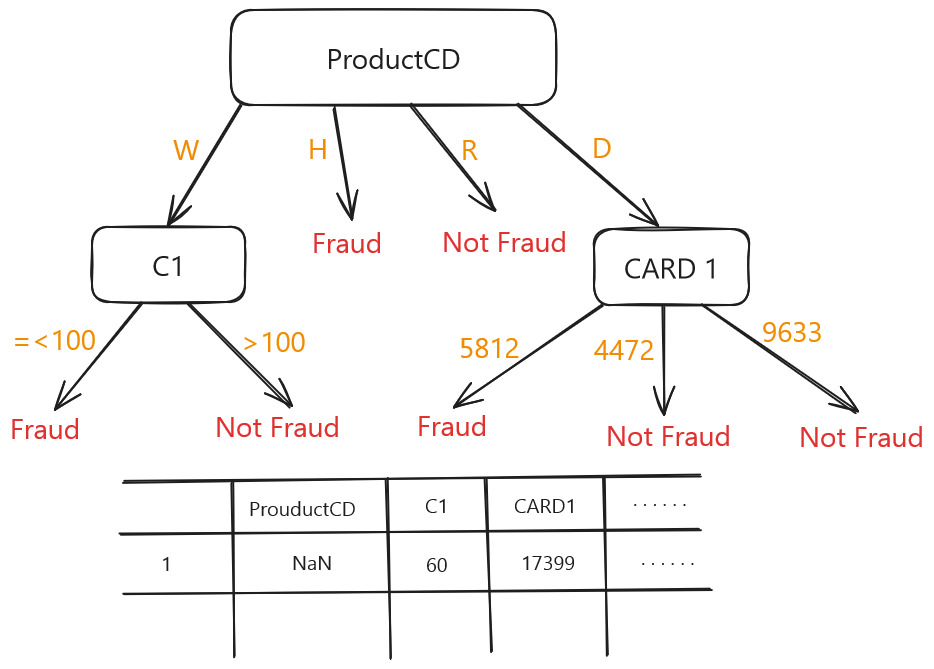
\includegraphics[width=1\linewidth]{Fig/NaN_test.jpg}
  \caption{A demo of 1 DT and 1 record}
\end{figure}


\subsection{Imbalanced data}
The dataset has 96.5\% of \textbf{not Fraud} transaction records, which is a significantly imbalanced (Table 2). To guarantee that each DT has enough \textbf{Fraud} transaction records while we randomly select 80\% of data in the training phase, we first split our dataset into "positive" set (Fraud) and "negative" set (Not Fraud). Then we extract 80\% from both sets as our training set, and the left 20\% as our validation set (Fig 2). By doing so, the algorithm is able to see a certain number of "Fraud" data in training phase, and have enough "Fraud" data for the validation phase.
\begin{table}[H]
    \centering        
    \begin{tabular}{r|r}
        Target & Percentage (\%)\\\hline
        Fraud& 3.50\\
        not Fraud& 96.50\\
    \end{tabular}
    \caption{Imbalanced target}
\end{table}

\begin{figure}[H]
  \centering
  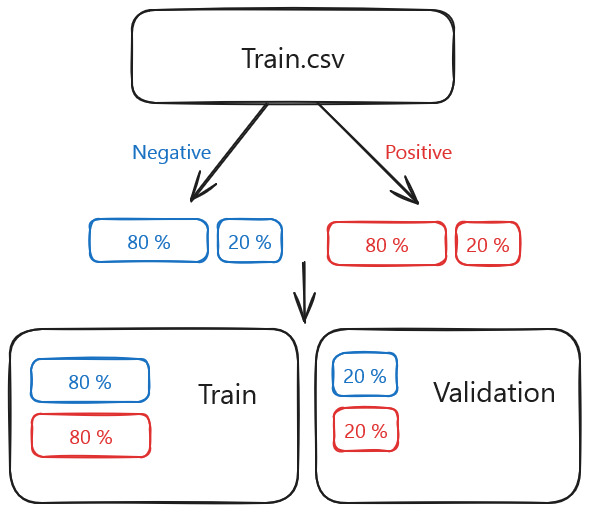
\includegraphics[width=1\linewidth]{Fig/Imblanced_data.jpg}
  \caption{Splitting data strategy}
\end{figure}





\section{Building a Tree}
\subsection{Information Gain Methods}
How to use information gain to build a tree has been discussed thoroughly in the class and from Micheal's book, we will not further discuss on it. In this report, we will focus on the experiments' results.\\\\
There are 3 information gain methods, 2 strategies dealing with missing values (Section 1.2). In total there are $3\times2 = 6$ combinations. For each combination, we did at least 9 experiments.\\\\ 
A subset balanced accuracy is shown in Table 3. For example, "MisEr3, Simulate, 67.81", means that this tree is using miss classification Information Gain method, and strategy 2 (Section 1.2) to deal with missing values in training phase. In the end, the validation balanced accuracy is 67.81\%.\\\\


\begin{table}[H]
    \centering        
    \begin{tabular}{r|r|r}
        Tree ID  & Missing value strategy & Balanced Accuracy (\%)\\\hline
        Gini0 & Filter &71.81\\
        Gini1 & Filter &71.02\\
        Gini2 & Filter &53.48\\\hline
        Gini3 & Simulate & 66.65\\
        Gini4 & Simulate & 58.45\\
        Gini5 & Simulate & 66.24\\\hline\hline
        Entropy0 & Filter & 57.25 \\
        Entropy1 & Filter & 65.24\\
        Entropy2 & Filter & 55.92\\\hline
        Entropy3 & Simulate & 67.86\\
        Entropy4 & Simulate & 63.00\\
        Entropy5 & Simulate & 58.62\\\hline\hline
        MisEr0 & Filter & 64.51\\
        MisEr1 & Filter & 50.93\\
        MisEr2 & Filter & 64.15\\\hline
        MisEr3 & Simulate & 67.81\\
        MisEr4 & Simulate & 68.68\\
        MisEr5 & Simulate & 66.71\\\hline\hline
        
    \end{tabular}
    \caption{Subset of trees' performance}
\end{table}

\begin{figure}[H]
  \centering

  \begin{subfigure}[t]{.45\linewidth}
    \centering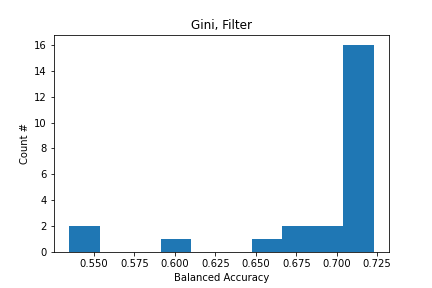
\includegraphics[width=1\linewidth]{Fig/Gini, Filter.png}
    \caption{Gini, Filter}
  \end{subfigure}
  \begin{subfigure}[t]{.45\linewidth}
    \centering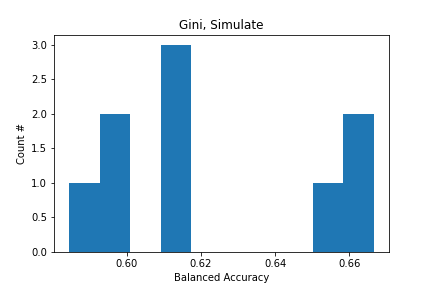
\includegraphics[width=1\linewidth]{Fig/Gini, Simulate.png}
    \caption{Gini, Simulate}
  \end{subfigure}\\

    \begin{subfigure}[t]{.45\linewidth}
    \centering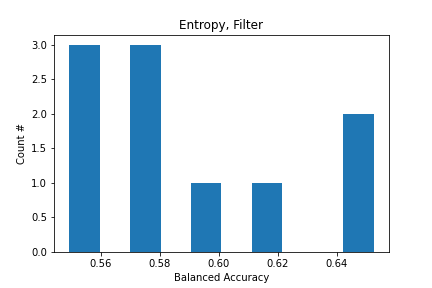
\includegraphics[width=1\linewidth]{Fig/Entropy, Filter.png}
    \caption{Entropy, Filter}
  \end{subfigure}
  \begin{subfigure}[t]{.45\linewidth}
    \centering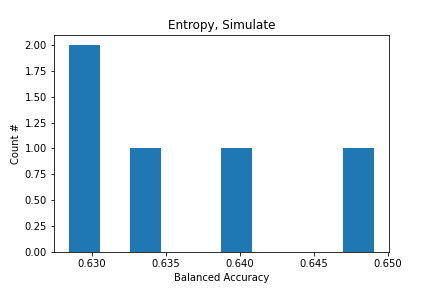
\includegraphics[width=1\linewidth]{Fig/Entropy, Simulate.png}
    \caption{Entropy, Simulate}
  \end{subfigure}\\

  \begin{subfigure}[t]{.45\linewidth}
    \centering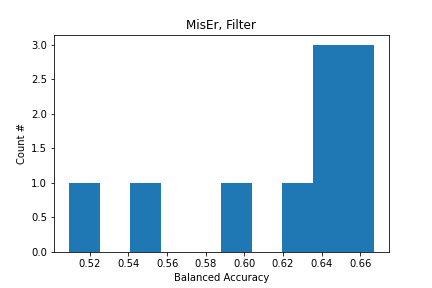
\includegraphics[width=1\linewidth]{Fig/MisEr, Filter.png}
    \caption{Miss classification, Filter}
  \end{subfigure}
  \begin{subfigure}[t]{.45\linewidth}
    \centering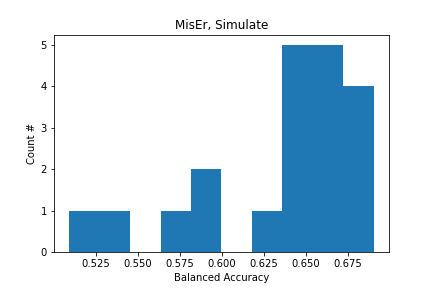
\includegraphics[width=1\linewidth]{Fig/MisEr, Simulate.png}
    \caption{Miss classification, Simulate}
  \end{subfigure}\\
  
  \caption{Histogram of Bal-Acc for each combination}
\end{figure}
The full experiments results is shown in Figure 3, using histograms. After the vertical comparison, Miss Classification is the least stable method for producing $\geq$0.6 balanced accuracy  trees, while Gini is the most stable one. The most interesting phenomenon is that using simulating data indeed increase the DT performance using Entropy or Miss Classification methods. But it will significantly decrease the balanced accuracy for Gini method. The reason is not discovered yet due to the time limit. \\\\
From these experiments, Random Forest is using "Gini" and "Filter" combination to generate trees. Also, from Figure 3. (a), the balanced accuracy of a single tree is roughly 0.7. If we want to have a 0.9 balanced accuracy for the final Random Forest, number of trees \textbf{n} should ensure:\\
${n\choose \frac{n}{2}}\times(1-0.7)^n \leq 0.1 \rightarrow n\geq 3$.\\
Since, we have already built 10+ trees with "Gini" and "Filter" combinations using random features and random 80\% records (following the strategy in Section 1.3), we will use all those trees whose balanced accuracy is greater than 0.65 for the Random Forest.\\\\
To test different method's influence to tree structure, we only used the same subset from the whole dataset and all features to do experiments. The strategy of dealing with missing data is also same for all three trees. \\\\
Figure 4 gives out the tree structure. Because some nodes have too many sub-branches ($>100$, \textbf{\# of Unique values} in Table 1), it's hard to plot the trees. Therefore, a Pandas DataFrame (df) is used to show the structure. \\\\
For example, Figure 4.(a) is a tree using Gini method. The root node of this tree is "card1" (Depth == 0). The root node's $1^{st}$-born child nodes are listed in Child\_Columns. For the $2^{nd}$ record (index is 1), this node's feature is 'ProductCD' (Column\_name), its parent node is 'card1' (Parent\_Col). This node is linked to the parent node by the edge 1008 (Parent\_Branch). Under this node, the Chi-Square test failed, hence this node has a Target value 0 and no child nodes (Child\_Columns is empty meaning that there is no edges coming out from this node). Whenever a record goes in this sub-branch, it will be assigned as "NotFraud" (Target == 0). \\\\
Figure 4.(b) is a tree using Entropy method. The root node of this tree is "addr1". For the $2^{nd}$ record, this node's feature is also "ProductCD", its parent node is "addr1". This node is linked to the parent node by the edge 100. Under this node, the Chi-Square test failed and the Target value is 0. For the $3^{rd}$ record, this node's feature is 'card1', its parent node is "addr1". This node is linked to the parent node by the edge 110. Under this node, the Chi-Square test failed and the Target value is 0. These 3 nodes together form 2 logic rules:\\
\textbf{Rule 1:} $addr1 == 100 \land ProductCD == C \rightarrow Target =NotFraud$\\
\textbf{Rule 2:} $addr1 == 110 \land card1 \in [1589,1726,2249,2803,3479,4812,7508,...] \rightarrow Target = NotFraud$\\
For the $4^{th}$ record, it is "ProductCD" again, its parent is "addr1", but this node is linked to the edge 122. And it passed Chi-Square test, therefore it has child nodes. But notice here, that its 3 sub-childs are its branches ([H,R,W]). Figure 4.(c) gives out these three child nodes' information. These 3 child nodes create additional logic rules:\\ 
\textbf{Rule 3:} $addr1 == 122 \land ProductCD == H \rightarrow Target =Fraud$\\
\textbf{Rule 4:} $addr1 == 122 \land ProductCD == R \rightarrow Target = NotFraud$\\
\textbf{Rule 5:} $addr1 == 122 \land ProductCD == W \rightarrow Target = NotFraud$\\\\

\begin{figure}[H]
  \centering

  \begin{subfigure}[t]{.9\linewidth}
    \centering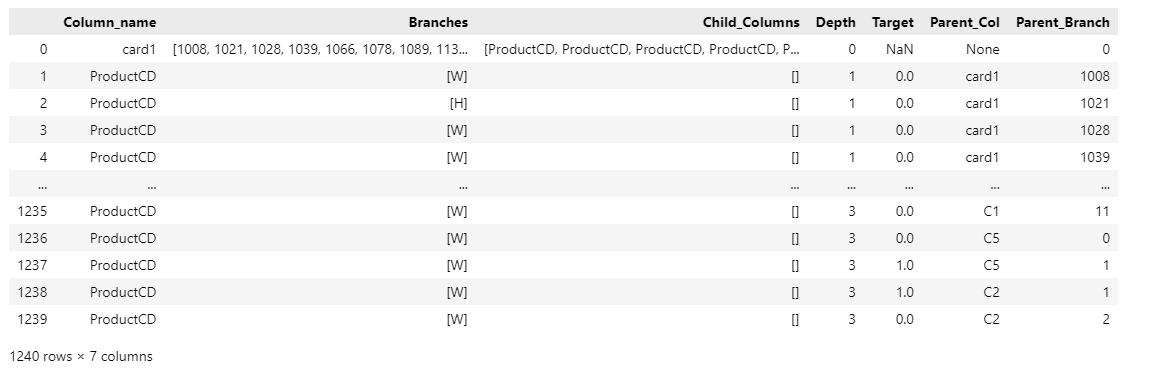
\includegraphics[width=1\linewidth]{Fig/Gini.png}
    \caption{Gini Tree}
  \end{subfigure}\\
  
  \begin{subfigure}[t]{.9\linewidth}
    \centering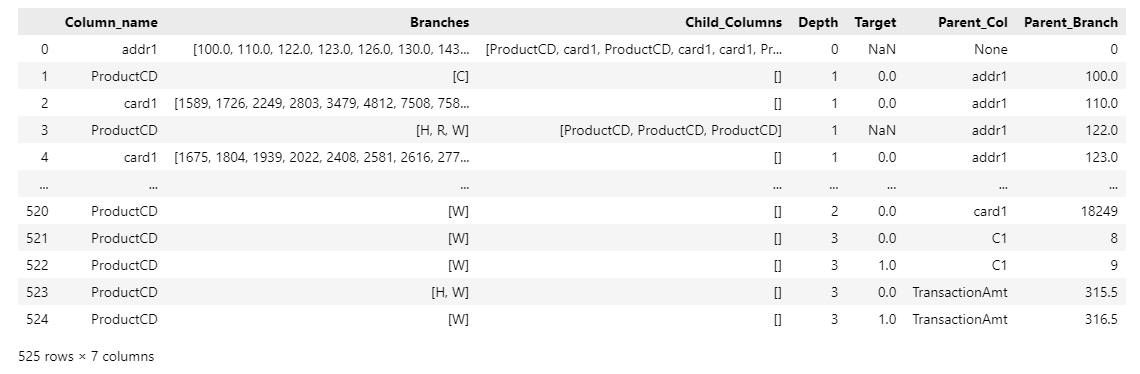
\includegraphics[width=1\linewidth]{Fig/Entropy.png}
    \caption{Entropy Tree}
  \end{subfigure}
  \begin{subfigure}[t]{.7\linewidth}
    \centering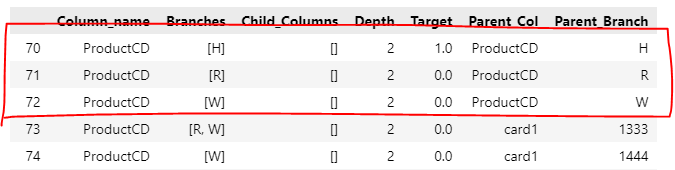
\includegraphics[width=1\linewidth]{Fig/Entropy_Sub.png}
    \caption{Entropy sub-Tree}
  \end{subfigure}
  \\

    \begin{subfigure}[t]{.9\linewidth}
    \centering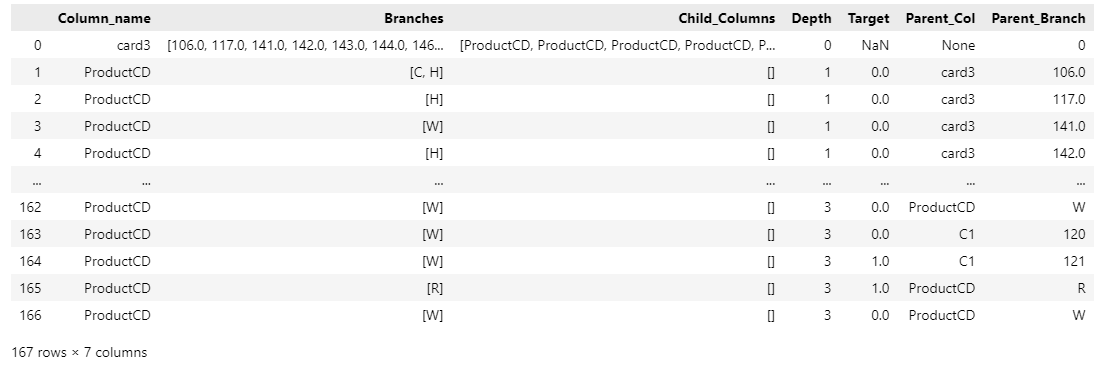
\includegraphics[width=1\linewidth]{Fig/MisEr.png}
    \caption{MisEr Tree}
  \end{subfigure}
  
  
  \caption{Different trees with different methods}
\end{figure}
In general, that's the structure of 3 trees using 3 different Information Gain methods. Only using the table view, we can tell the difference among these trees' structures. Miss Classification generate trees with least amount of nodes (166). Gini index has greatest amount of nodes. Their height are all 3 (although I set the Max-Depth = 5). We can also tell that Gini's tree is wider compared to the others. This difference is caused by different ways of calculating Information Gain. Actually, Gini index choose \textbf{card1} as the root node, Entropy choose \textbf{addr1}, while Miss Classification choose \text{card3}. From Table 1, \textbf{card1} has significantly larger sub-branches. Even though I let the Information Gain function to use the Gain-Ratio when it detect more than 200 sub-branches, \textbf{card1} still had the best Gain-Ratio for Gini index, but not for the other two. 



\subsection{$\alpha$ value}

To overcome the over-fitting problem, Chi-square test is used whenever the DT trid to expand under one node. The $\alpha$ value affect the basic Chi-value (which value we choose from the Chi-Table). Because the degree of freedom under each node won't change, the basic Chi-value is only influence by the $\alpha$ we choose. With a higher $\alpha$, we have less confidence interval (1-$\alpha$), and a lower basic Chi-value. Let Chi-Node represent the Chi-square of our targeted node. When Chi-Node $>$ basic Chi-value, we said the node pass the Chi-square test, and let the tree keep growing under this node.\\\\
From this process, we can tell that $\alpha$ value can affect the depth of the tree. And the depth of the tree affect the accuracy and over-fitting problem. Given the constraint that our tree's maximum depth = 5, and we have 25 features, it's reasonable to make a conclusion that the tree won't encounter over-fitting problem easily. Hence, we make a hypothesis here $h_0$: higher $\alpha \rightarrow$ lower balanced accuracy $\land$ deeper tree.\\\\
An experiment is done using the same subset from the whole dataset, Gini index as Information Gain, strategy 1  (Section 1.2) to deal with missing values. results 



\section{Save a DT to a DataFrame (DF)}



In our project, with alpha 0.05, we got 0.71 balanced accuracy. 



\section{Appendix}



\end{document}
